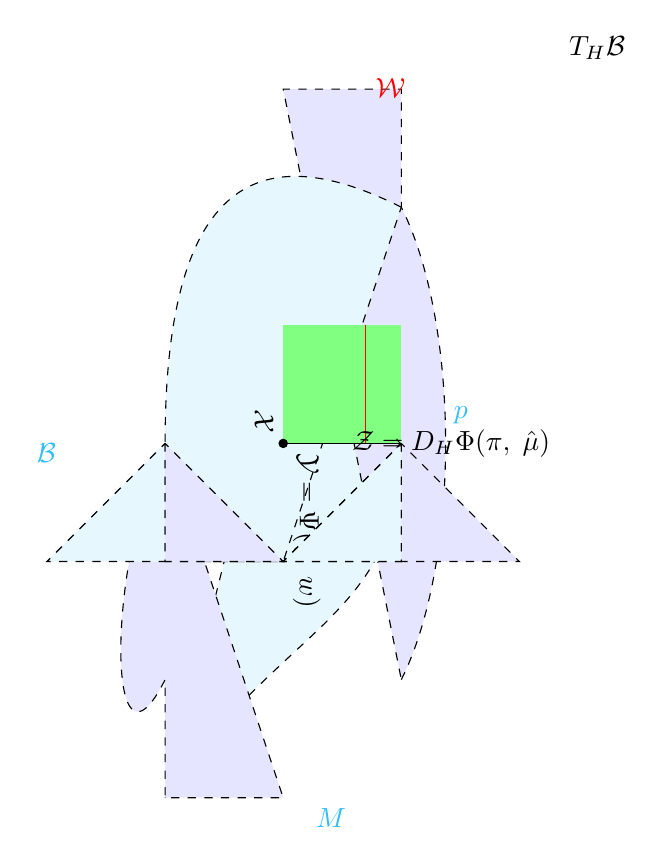
\begin{tikzpicture}[scale=1.5]
    \draw[dashed=cyan!80, fill=cyan!10] (-1,-2) .. controls (0,-0.5) and (1,-0.5) .. 
        (1,1) -- ++(0,1) -- ++(-1,0) -- cycle;
    \draw[dashed=blue, fill=blue!10] (1,-1) .. controls (1.5,0) and (1.5,2) ..
        (1,3) -- ++(0,1) -- ++(-1,0) -- cycle;
    \draw[dashed=cyan!80, fill=cyan!10] (1,3) .. controls (0,3.5) and (-1,3.5) ..
        (-1,1) -- ++(0,-1) -- ++(1,0) -- cycle;
    \draw[dashed=blue, fill=blue!10] (-1,1) .. controls (-1.5,0) and (-1.5,-2) ..
        (-1,-1) -- ++(0,-1) -- ++(1,0) -- cycle;
    \draw[dashed=cyan!80, fill=cyan!10] (1,1) -- ++(0,-1) -- ++(-1,0) -- cycle;
    \draw[dashed=blue, fill=blue!10] (-1,1) -- ++(0,-1) -- ++(1,0) -- cycle;
    \path[fill=green!50] (0,1) -- ++(1,0) coordinate[pos=.7] (aux) -- ++(0,1) coordinate[pos=.7] (aux)
     -- ++(-1,0) coordinate[pos=.3] (aux) -- cycle;
    \draw[red] (aux) -- ++(0,-1);
    \node[right,red] at (aux|-current bounding box.north) {$\mathcal{W}$};
    \filldraw (0,1) node[above right,rotate=-90,anchor=south west]{$\mathcal{Y}=\Psi(\xi,\;w)$}
      circle[radius=1pt] node[below left,rotate=-90]{$\mathcal{X}$};
    \draw[dashed=cyan!80, fill=cyan!10] (-1,1) -- ++(0,-1) -- ++(-1,0) -- cycle;
    \draw[dashed=blue, fill=blue!10] (-1,1) -- ++(0,-1) -- ++(1,0) -- cycle;
    \node[cyan!80,above] at (current bounding box.east){$p$};
    \node[cyan!80,below] at (current bounding box.west){$\mathcal{B}$};
    \draw[dashed=cyan!80, fill=cyan!10] (1,1) -- ++(0,-1) -- ++(-1,0) -- cycle;
    \draw[dashed=blue, fill=blue!10] (1,1) -- ++(0,-1) -- ++(1,0) -- cycle;
    \draw[->] (0,1) -- node[right]{$\mathcal{Z}=D_{H}\Phi(\pi,\;\hat{\mu})$} (1,1);
    \node[above right] at (current bounding box.north east){$T_{H}\mathcal{B}$};
    \node[cyan!80,below] at (current bounding box.south){$M$};
\end{tikzpicture}